\chapter{Implementácia riešenia}
\label{chap:SixthChapter}
\section{Výber technológií a nástrojov}
\subsection{Kritériá výberu}
\begin{hyphenrules}{nohyphenation}
Rozhodnutie pri výbere technológie padlo na \texttt{C\#} a \texttt{.NET 8} kvôli robustnej podpore pre webové služby a~pokročilým vedomostiam daného jazyka. Pre analýzu a~spracovanie PDF dokumentov boli použité knižnice \texttt{ImageMagick} a~\texttt{OpenCV}. Náš softvér cieli na operačný system Windows 10.

\subsection{Použité technológie}
\begin{itemize}
    \item Jazyk: \texttt{C\#}
    \item Framework: \texttt{.NET 8}
    \item API: Minimal API v \texttt{.NET 8}
    \item Použité knižnice (NuGety): 
    \begin{itemize}
        \item Coverlet \cite{coverlet}
        
        - Použitý pre štatistiku nad pokrytím kódu testami.
        \item ErrorOr \cite{error-or}
        
        - Menší NuGet, ktorý pomáha riešiť vyhadzovanie výnimiek a miesto nich poskytuje intuitívny prístup k návratovej hodnote.
        \item FluentValidation \cite{fluentvalidation}

        - Intuitívny spôsob validácie vstupov a validácie pri tvorbe objektov.
        \item Magick.NET \cite{magicknet}

        - Nadstavba nad ImageMagick, vhodný pri manipulácii a úprave obrázkov, v našom prípade použitý pri konverzii PDF dokumentov do formátu vhodného pre ďalšie procesy.
        \item Mapster \cite{mapster}

        - Umožňuje jednoduché mapovanie objektov, primárne použitý pri mapovaní HTTP requestov na objekty, s ktorými ďalej pracuje aplikácia.
        \item MediatR \cite{mediatr}

        - Umožňuje implementáciu vzoru mediátora, čím zjednodušuje komunikáciu medzi komponentami aplikácie tým, že sprostredkováva požiadavky a notifikácie medzi odosielateľmi a prijímateľmi bez ich vzájomnej závislosti.

        \item Entity Framework Core \cite{efcore}

        - ORM knižnica pre .NET, ktorá umožňuje pracovať s databázami, umožňuje mapovanie medzi databázovými tabuľkami a triedami v~aplikácii.

        \item Microsoft DependencyInjection \cite{dependency-injection}

        - Poskytuje vstavanú podporu pre Dependency Injection, umožňuje automatickú správu závislostí medzi jednotlivými komponentami aplikácie.

        \item OpenCvSharp4 \cite{opencv}

        - Nadstavba nad OpenCV pre .NET.

        \item xUnit \cite{xunit}

        - Testovací framework slúžiaci na jednoduché testovanie aplikácie.
        
    \end{itemize}
\end{itemize}

Aplikácia je vybavená aj SQLite\cite{sqlite} databázou, ktorá poskytuje ľahkú a~kompaktnú relačnú databázu a umožňuje lokálne ukladanie a spracovanie dát bez potreby samostatného servera.

\section{Architektúra a dizajn systému}
\subsection{Architektúra riešenia}
Architektúra našej aplikácie je založená na tzv. Domain-Driven Design, ktorá je popísana v knihe od Scotta Millett-a a Nicka Tune-a, \textit{Patterns, Principles, and Practices of Domain-Driven Design}\cite{millett2015ddd}. Domain-Driven Design (DDD), resp. Domain-Driven architecture je často označovaný aj ako vrstvová architektúra, cibuľová architektúra či "čistá" architektúra. 
\newline

Vrstvová architektúra je rozdelená do viacerých vrstiev, ktoré sa vzťahujú na~rozličné aspekty daného systému. Každá vrstva má jasnú a~špecifickú úlohu a~vrstvy sa navzájom ovplyvňujú len jedným smerom.

Hlavnými prvkami vrstvovej architektúry sú:
\begin{enumerate}
    \item Prezenčná vrstva: Zodpovedá za interakciu s uživateľom,
    \item Aplikačná vrstva: Zodpovedá za implementáciu biznisovej logiky, ktorá sa vzťahuje na uživateľské požiadavky,
    \item Servisná vrstva: Slúži na poskytovanie služieb, ktoré sú potrebné pre aplikáciu,
    \item Infraštruktúrna vrstva: Zodpovedá za správu a komunikáciu s externými zdrojmi,
    \item Perzistentná vrstva: Slúži na komunikáciu s perzistentne uloženými dátami, databázou.
\end{enumerate}


\begin{figure}[H]
    \centering
    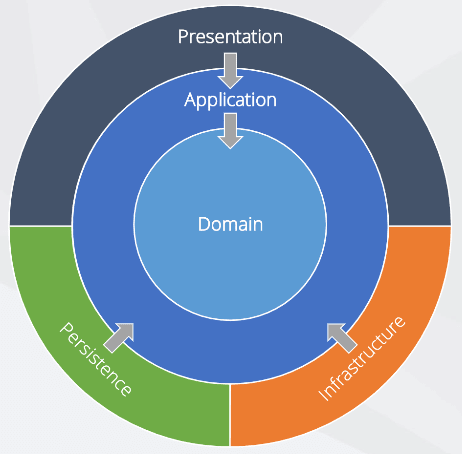
\includegraphics[width=0.4\linewidth]{img/onion.png}
    \caption{Grafické znázornenie cibuľovej architektúry\cite{danielrusnok}}
    \label{fig:6.1}
\end{figure}
Každá vrstva je navrhnutá tak, aby bola izolovaná od ostatných vrstiev. Vrstvy medzi sebou komunikujú pomocou rozhraní a preto zmeny v jednej vrstve nevytvárajú nepredvídateľné zmeny v iných vrstvách. Pomocou rozhraní definujeme, čo dané vrstvy môžu a nemôžu robiť.
\newline

Najväčšími výhodami tejto architektúry sú modularita, odolnosť voči zmenám a jednoduchosť pri návrhu samotnej aplikácie.

\section{Detaily implementácie}

\subsection{Pomocné aplikácie a testovacie projekty}
\label{chap:6.3.1}
V rámci projektu DAPP\cite{lukassalak} sme implementovali pomocný projekt s~názvom \texttt{ManualCheckerUtility}. Pri spustení automaticky stiahne dokumenty, ktoré sú následne po jednotlivých stránkach zobrazované uživateľovi. V pravej strane sa nachádza niekoľko možností, ktoré užívateľ môže zvoliť a tie sa následne postupne ukladajú do štatistiky. 

\begin{figure}[H]
    \centering
    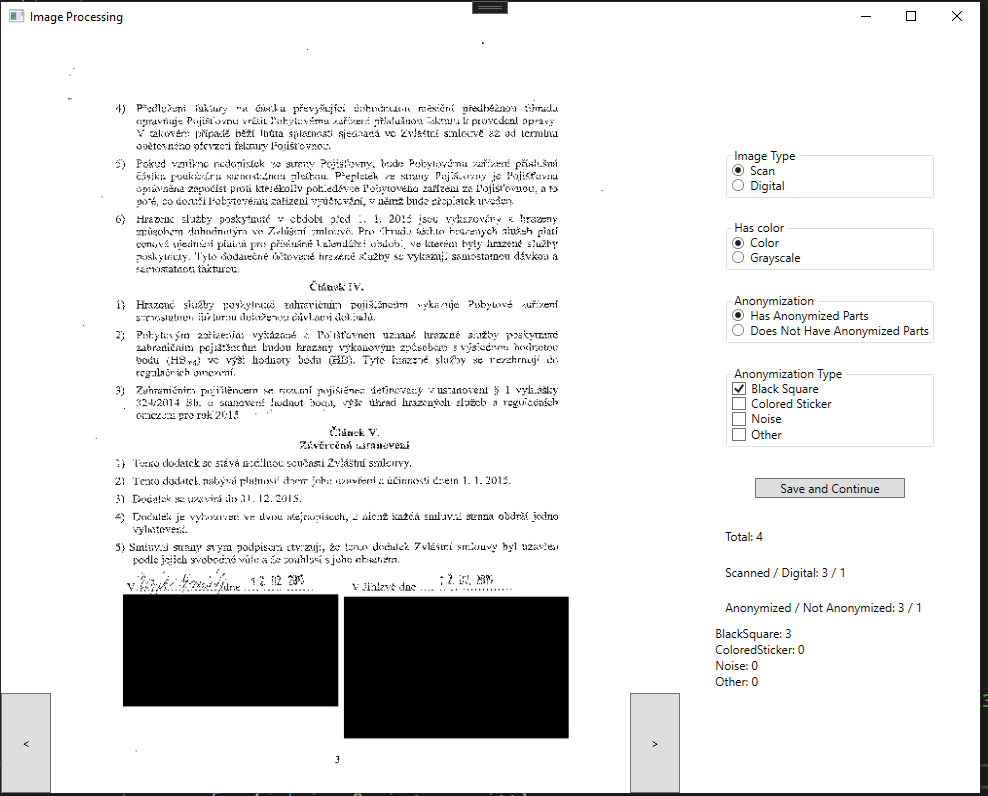
\includegraphics[width=0.9\linewidth]{img/image_proc.png}
    \caption{Ukážka grafického rozhrania \texttt{ManualCheckerUtility}}
    \label{fig:6.2}
\end{figure}

Súčasťou riešenia okrem testov je aj projekt s~názvom \texttt{GenerateTestResults}. Jedná sa o jednoduchý skript, ktorý umožňuje rýchlo generovať výsledky s~aktuálnym kódom a ukladať tieto výsledky sekvenčne s prebiehajúcimi zmenami. 
Skript si na začiatku vytvorí WebClient hlavného programu nesúceho názov API2. API2 je druhá verzia projektu API, ktorá bola vzhľadom na použitú architektúru zastaraná a preto sme sa rozhodli prejsť na tzv. minimal api \cite{aspnetcore}. Následne po inicializácii WebClient-a prevoláva toto API s requestami obsahujúcimi jednotlivé dokumenty z našej testovacej sady. Po vrátení response sa tieto dáta dekomponujú z~formátu JSON a uložia na disk, kde ich je potom možné prehliadať. Ukladajú sa originálne snímky, analyzované snímky a percentá anonymizácie pre jednotlivé strany.

\subsection{Realizácia algoritmu}
Hlavným projektom, ktorý je nosnou časťou našej aplikácie okrem samotného API a jeho častí, je projekt s názvom \texttt{DAPPAnalyzer}, ktorý obsahuje algoritmus na detekciu anonymizovaných častí.
\newline

Súbor \texttt{PDFAnalyzer.cs} obsahuje implementáciu triedy \texttt{PDFAnalyzer}, ktorá implementuje niekoľko metód. Hlavnou a vstupnou metódou je metóda \texttt{Task<AnalyzedResult> AnalyzeAsync(DappPDF pdf);}, ktorá je jedinou verejnou metódou tejto triedy. Jej funkciou je paralelne pre každú stranu z~parametru pustiť privátnu funkciu \texttt{AnalyzePage} a následne vrátené výsledky uložiť do modelu \texttt{AnalyzedResult}, ktorý obsahuje okrem identifikačných znakov, akými sú názov dokumentu, url či počet strán dokumentu, samotné výsledky analýzy. Tými sú:
\begin{itemize}
    \item \texttt{containsAnonymizedData} : boolean, ktorý určuje, či boli detegované anonymizované oblasti,
    \item \texttt{anonymizedPercentagePerPage} : slovník, kde kľúč je index strany a~hodnota je percento anonymizácie pre danú stranu,
    \item \texttt{originalImages} : slovník, kde kľúč je index strany a hodnota je \texttt{byte[]}, teda snímok danej strany uložený ako \texttt{byte array},
    \item \texttt{anonymizedImages} : rovnako ako pri \texttt{originalImages}, až na to, že \texttt{byte[]} obsahuje výslednú "masku", teda obraz, kde sú znázornené len anonymizované oblasti.
    
\end{itemize}

Na ďalšej strane prikladáme zdrojový kód tejto funkcie. Pre ešte bližšie detaily prikladáme v prílohe zdrojový kód, kde je dostupná celá implementácia so všetkými pomocnými skriptami a testovacími súbormi.
\newpage
\begin{lstlisting}
internal static Mat GetAnonymizedParts(
    Mat img, 
    int erodeValue = 8, 
    int dilateValue = 4)
{

    var coloredPixels = ColoredPixels(img);
    // Increase their saturation 
    var imgSaturatedColors = img;
    if (coloredPixels.Count != 0)
    {
       imgSaturatedColors = 
            IncreaseSaturation(img, coloredPixels, 100);
    }
    // Create structuring element
    Mat se = 
        Cv2.GetStructuringElement(
            MorphShapes.Rect, 
            new Size(3, 3));
    var dilated = Dilate(imgSaturatedColors, se);

    var dilated_threshold = Threshold(dilated, 20);
    var dilated2 = Dilate(dilated_threshold, se);


    var result = dilated2;
    for (int i = 0; i < erodeValue; i++)
    {
        result = Erode(result, se);
    }
    for (int i = 0; i < dilateValue; i++)
    {
        result = Dilate(result, se);
    }

    return Threshold(result,127);
}
\end{lstlisting}

Pre jednoduchšiu čitateľnosť je na ďalšej strane znázornený stavový diagram.
\newpage
\begin{figure}[H]
    \centering
    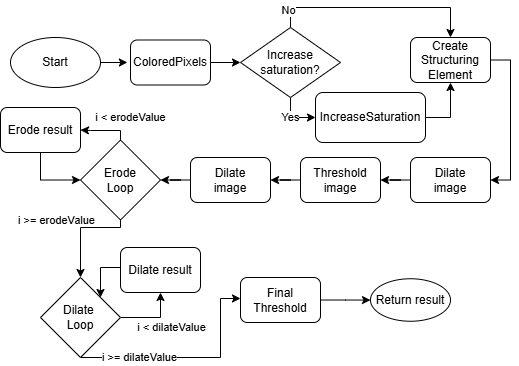
\includegraphics[width=0.9\linewidth]{img/diagram.png}
    \caption{Diagram funkcie \texttt{GetAnonymizedParts}}
    \label{fig:6.3}
\end{figure}
\subsection{Testovanie}
Vývoj prebiehal na verzovacom systéme git a je uložený na školskej inštancii gitlab \cite{lukassalak}, v repozitári je pripravená CI/CD pipeline na automatický build a automatické spustenie testov. Na obrázku \ref{fig:6.4} vidíme pokrytie testami sprostredkované frameworkom coverlet\cite{coverlet}.

\begin{figure}[H]
    \centering
    \fbox{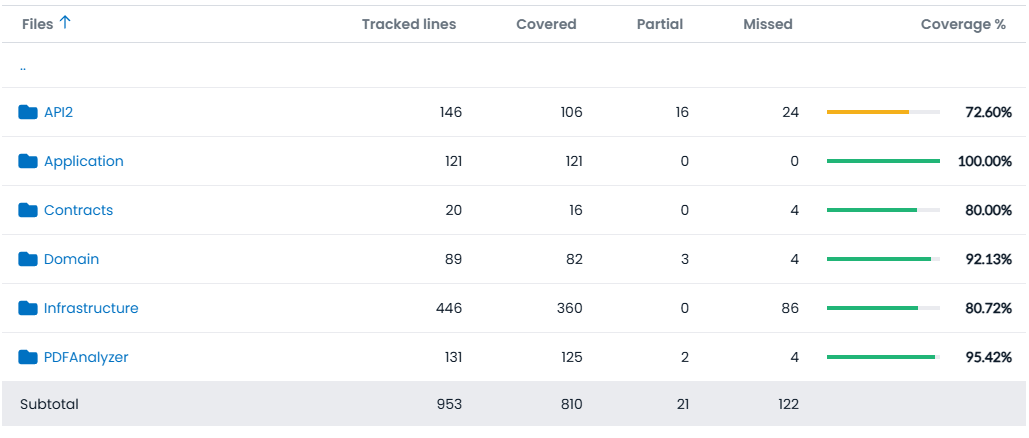
\includegraphics[width=0.7\linewidth]{img/pokrytie.png}}
    \caption{Pokrytie testov jednotlivých častí softvéru\cite{coverlet}}
    \label{fig:6.4}
\end{figure}
\end{hyphenrules}